\begin{figure}[H]
    \centering
    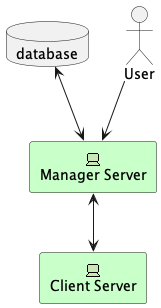
\includegraphics[height=0.4\textheight]{./part/Proyecto_ejecutivo/memoria_descriptiva/descripcionDelProyecto/manager/uml/managerServerConcept}
    \caption[Diagrama componentes]{}\label{fig:managerServerConcept}
\end{figure}

\subparagraph{Dominio}

En el diagrama UML~\ref{fig:managerDomain} vemos que el dominio de Manager se compone de dos modulos: uno para las tareas y otro para los resultados. Vamos a ir explicando uno por uno:

\begin{itemize}
    \item Core
    \begin{itemize}
        \item Id todos los ids extenderan de este id, contiene un uuid, no sabemos que paquete usaremos para generarlos, es una de las pocas dependencias externas que vamos a tener dentro del dominio y queremo encapsularla lo máximo posible por si hubera que cambiarla. Además de esta forma los ids de las entities no se confunden en su tipo. si por ejemplo buscas una task mediante un id que corresponde a un result, si fueran del mismo tipo daría lugar a confusión porque no lo encontraríamos pero no nos advertiría de nuestro error
        \item Event todos los eventos del sistema extenderan del evento este
    \end{itemize}
    \item Task
    \begin{itemize}
        \item TaskId
        \item Host: es un Value Object compuesto por el valor del host, es un string pero el Value Object garantiza que es un valor válido, si no devuelve un error
        \item Port: es un Value Object compuesto por el valor del puerto, es un string pero el Value Object garantiza que es un valor válido, si no devuelve un error
        \item CommunicationMode: es un enum para expresar esa tarea de las formas de comunicación posibles que hay entre dos servidores cual sera la utilizada
        \begin{itemize}
            \item UNARY
            \item SERVER\_STREAM
            \item CLIENT\_STREAM
            \item BIDIRECTIONAL
        \end{itemize}
        \item ExecutionMode: es un enum
        \begin{itemize}
            \item MANUAL
            \item AUTOMATIC
        \end{itemize}
        \item Status: es un enum
        \begin{itemize}
            \item PENDING
            \item RUNNING
            \item SUCCESSFUL
            \item FAILED
        \end{itemize}
        \item Step: cada tarea puede componerse en distintos pasos. Por ejemplo queremos poder poner en marcha el motor durante 15 segudos y luego llevarlo a una posición de inicio
        \begin{itemize}
            \item StepId
            \item sentence: será un string de contenido libre que el servidor cliente ejecutará en su sistema, dependerá de él tener instalado dicho programa y corroborar que la sintaxis es la correcta
        \end{itemize}
        \item TaskCreatedEvent. Cuando se cree una tarea se emitirá un evento, habrá un manejador de eventos que actuará en consecuencia. Si es una tarea automatizada y el loop de ejecución está parado lo pondrá en marcha.
        \item TaskModifiedEvent: si una tarea es modificada se emitirá un evento, habrá un manejador de eventos que actuará en consecuencia. Si la tarea vuelve a ser puesta a pending, es automatizada y el loop de ejecución está parado lo pondrá en marcha
        \item TaskDeletedEvent: si una tarea es modificada se emitirá un evento, habrá un manejador de eventos que actuará en consecuencia.
    \end{itemize}

\end{itemize}

\begin{figure}[H]
    \centering
    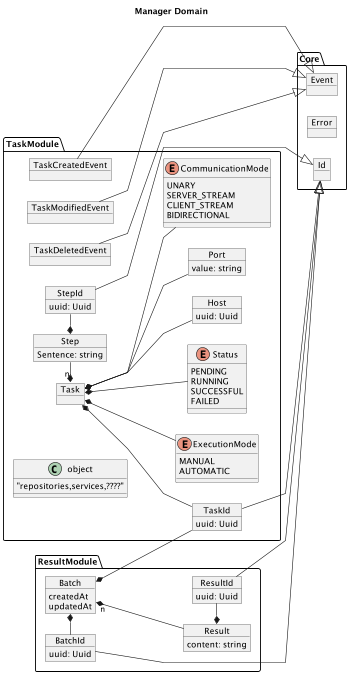
\includegraphics[height=0.4\textheight]{./part/Proyecto_ejecutivo/memoria_descriptiva/descripcionDelProyecto/manager/uml/managerDomain}
    \caption[Diagrama de objetos de dominio]{}\label{fig:managerDomain}
\end{figure}

\subparagraph{casos de uso}

Vamos a describir los casos de uso que podrán ejecutarse en el programa manager

\textbf{crear tarea}

\begin{figure}[H]
    \centering
    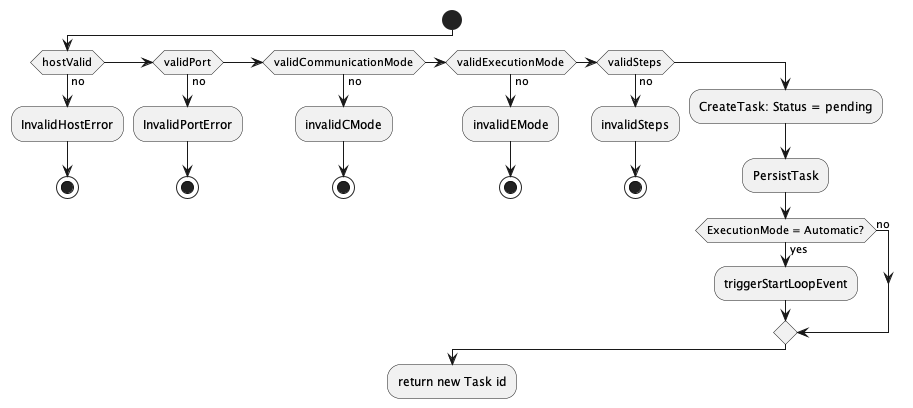
\includegraphics[height=0.3\textheight]{./part/Proyecto_ejecutivo/memoria_descriptiva/descripcionDelProyecto/manager/uml/createTaskUseCase}
    \caption[Diagrama de objetos de dominio]{}\label{fig:createTaskUseCase}
\end{figure}

\textbf{obtener tarea}

\begin{figure}[H]
    \centering
    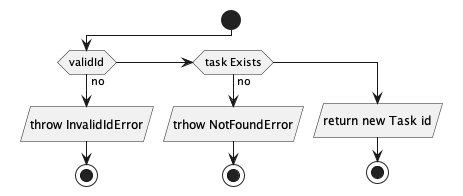
\includegraphics[height=0.3\textheight]{./part/Proyecto_ejecutivo/memoria_descriptiva/descripcionDelProyecto/manager/uml/getTaskUseCase}
    \caption[Diagrama de objetos de dominio]{}\label{fig:getTaskUseCase}
\end{figure}

\textbf{listar tareas}

Uno de los puntos más amplios en una API CRUD es el filtrado de datos. No entra dentro del ámbito de este proyecto crear un sistema de filtrado que incluya la paginación. En este caso habría que crear una nomenclatura de filtros de cara al usuario y un sistema que los procese, devolviendo error ante un filtro erroneo o el listado de tareas que responda a dicho filtro. En nuestro caso devolveremos todas las tareas.

\textbf{actualizar tareas}

\begin{figure}[H]
    \centering
    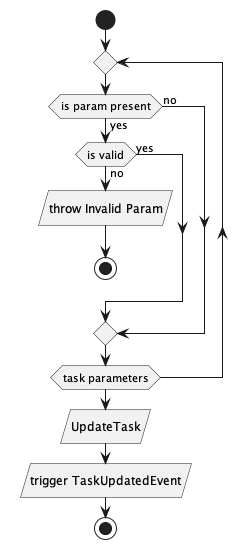
\includegraphics[height=0.5\textheight]{./part/Proyecto_ejecutivo/memoria_descriptiva/descripcionDelProyecto/manager/uml/updateTaskUseCase}
    \caption[Diagrama de objetos de dominio]{}\label{fig:updateTaskUseCase}
\end{figure}

\textbf{eliminar tareas}

\begin{figure}[H]
    \centering
    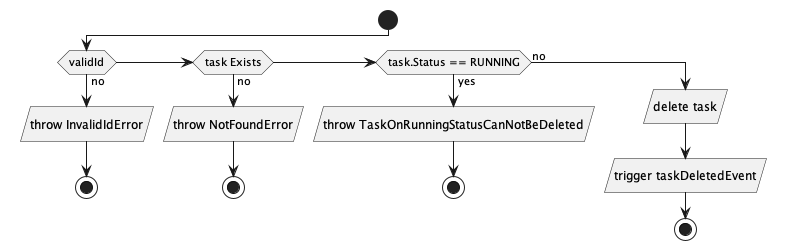
\includegraphics[height=0.2\textheight]{./part/Proyecto_ejecutivo/memoria_descriptiva/descripcionDelProyecto/manager/uml/deleteTaskUseCase}
    \caption[Diagrama de objetos de dominio]{}\label{fig:deleteTaskUseCase}
\end{figure}

\textbf{TaskEventHandler}

tanto en TaskCreatedEvent como TaskUpdatedEvent el handler va a ser el mismo. TaskDeletedEvent lo dejaremos en este diseño inicial.

\begin{figure}[H]
    \centering
    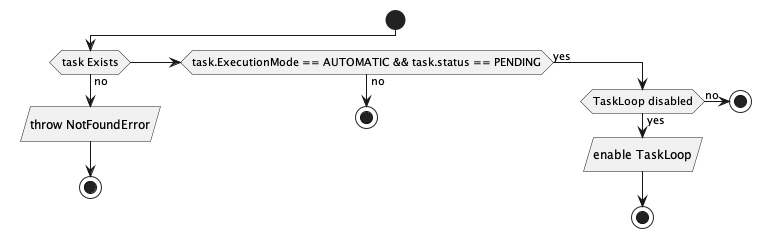
\includegraphics[height=0.2\textheight]{./part/Proyecto_ejecutivo/memoria_descriptiva/descripcionDelProyecto/manager/uml/taskEventHandlerUseCase}
    \caption[Diagrama de objetos de dominio]{}\label{fig:taskCreatedEventHandtaskEventHandlerUseCaselerUseCase}
\end{figure}

\textbf{TaskLoop: ejecutar tareas automáticas pendientes}

Una vez que el TaskEventHandler ponga en marcha el TaskLoop este obtendrá de base de datos todas las tareas automáticas pendientes y iterando sobre ellas lanzará un hilo de ejecución para ejecutarlas. Una vez terminadas todas volverá a intentar obtener tareas pendientes ya que en el periodo que haya estado ejecutandolas pueden haberse introducido nuevas. Si no hay más tareas pendientes el loop se desactivará.

Un punto a mencionar de este Task loop es que se implementará en aplicación porque aquí intervendrán todavía puntos de la aplicación y la tecnología que no están investigados y son complejos. Es donde esta arquitectura mostrará toda su flexibilidad y fiabilidad de cara a proteger los elementos básicos de la aplicación de los cambios.

Una vez desarrollado, o puede que incluso durante el mismo desarrollo habrá en este proceso muchos conceptos que descubriremos core de la aplicación y debieran ser dominio, pero como tenemos que descubrirlos vamos a implementarlos en aplicación haciendo uso de interfaces de infraestructura y de elementos de dominio. Si vemos claramente que algo puede convertirse en dominio lo introduciremos.

\sout{Será el único punto en donde una interfaz de dominio será implementada por un elemento de aplicación en vez de infraestructura.} \textcolor{red}{El diseño de esto es complejo y todavía no lo tengo. Event handler necesita todo para crearse?}

\begin{figure}[H]
    \centering
    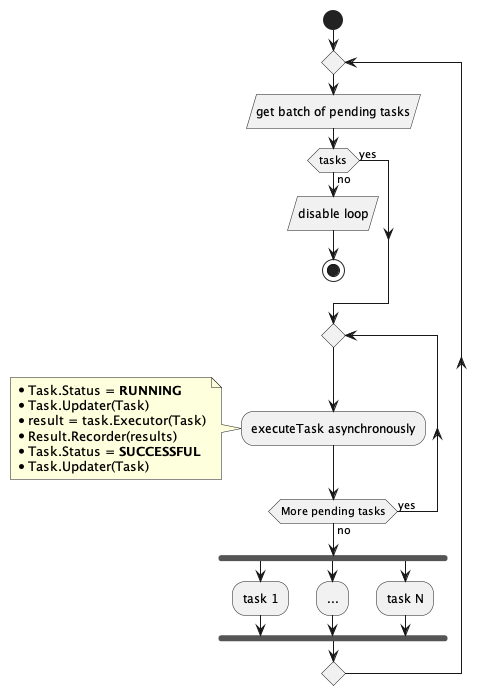
\includegraphics[height=0.3\textheight]{./part/Proyecto_ejecutivo/memoria_descriptiva/descripcionDelProyecto/manager/uml/executeTaskLoop}
    \caption[Diagrama de objetos de dominio]{}\label{fig:executeTaskLoop}
\end{figure}

\textbf{Create Batch}

\subparagraph{estructura de carpetas}

Una de las partes mas importantes de un proyecto de software es que la estructura de carpetas hable sobre cómo está diseñado el software, sobre de qué va el software. qué es lo que hace y sobre que componentes interactua

En el proyecto constará de 4 carpetas principales
\dirtree{%
    .1 Project .
        .2 Adapter.
        .2 Application.
        .2 Domain.
        .2 Bootstrap.
}

Bootstrap será donde hagamos la composición de la aplicación, es decir la inyección de dependencias.

Vamos a desplegar la estructura capa por capa

\textbf{Adapters}

\dirtree{%
.1 Adapter.
    .2 in.
        .3 GRPC.
            .4 CreateEntityGrpcCall.
        .3 Console.
            .4 CreateEntityTerminalCommand.
    .2 out.
        .3 Email.
            .4 SendEmailOnCreationImplementation (*1).
        .3 Mysql.
            .4 SaveEntityImplementation (*2).
}

\textbf{Aplicación}

\dirtree{%
.1 Application.
    .2 Port.
        .3 in.
            .4 Entity.
                .5 CreateUseCase.
                    .6 CreateCommand.
                        .7 CreateCommand (using sendEmail param in this example).
                        .7 CreateUseCase.
                    .6 SomeEventHandler.
                        .7 CreationEvent.
                        .7 CreationEventUseCase.
        .3 out.
            .4 Email.
                .5 SendEmailConCreation (interface for *1).
}

\textbf{Dominio}

\dirtree{%
.1 Domain.
    .2 Core.
        .3 Id.
        .3 Event.
        .3 Error.
    .2 Task.
        .3 Id.
        .3 Task.
        .3 Host.
        .3 Port.
        .3 CommunicationMode.
        .3 ExecutionMode.
        .3 Status.
        .3 Step.
            .4 Id.
            .4 StepEntity.
            .4 StepVo.
            .4 Repository.
                .5 Find.
                .5 Save.
                .5 Search.
                .5 Delete.
                .5 Update.
            .4 Service.
                .5 Finder.
                .5 Creator.
                .5 Updater.
                .5 Eraser.
                .5 Searcher.
        .3 Repository.
            .4 Find.
            .4 Save.
            .4 Search.
            .4 Delete.
            .4 Update.
        .3 Service.
            .4 Finder.
            .4 Creator.
            .4 Updater.
            .4 Eraser.
            .4 Searcher.
    .2 Result.
}

Queda pendiente implementar aplicación e infraestructura.
